\documentclass[tikz, border = 2pt]{standalone}

%---------------------------------------------------------------------------%
% PACKAGES                                                                  %
%---------------------------------------------------------------------------%

%----- MATH
%---------------------------------------------------------------------------%
\usepackage{amsmath, amssymb}

%----- FIGURES
%---------------------------------------------------------------------------%
\usepackage{pgfplots}
\pgfplotsset{compat=1.13}

\begin{document}

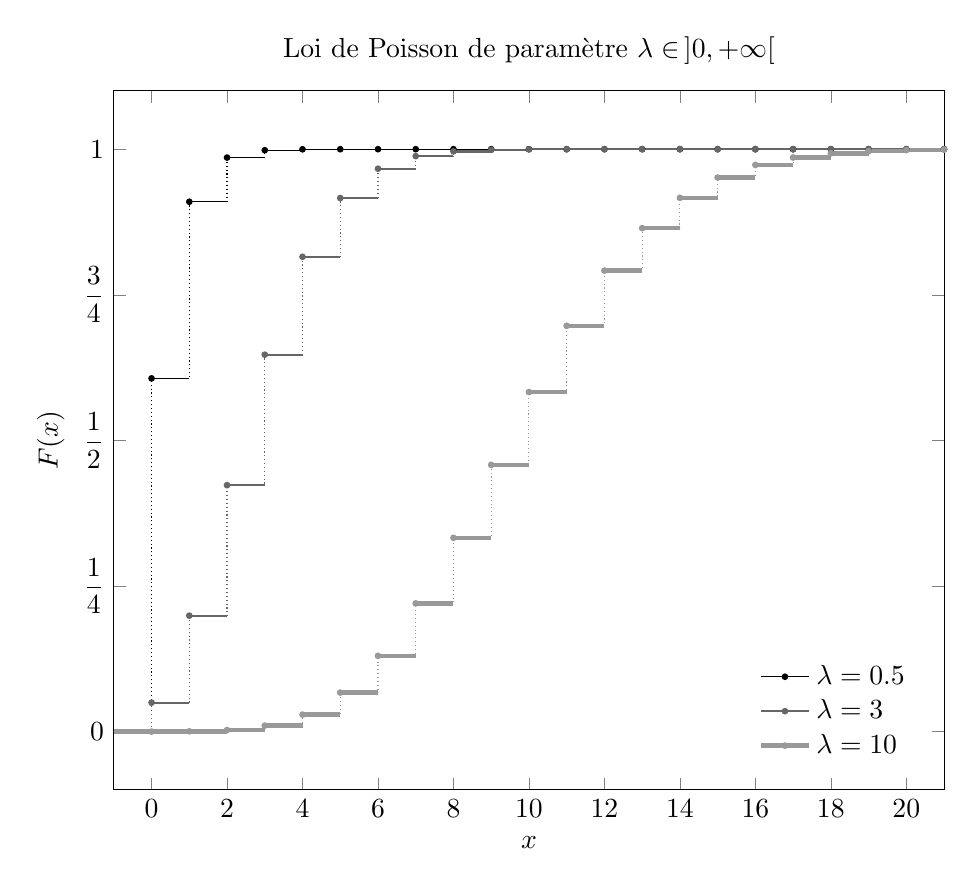
\begin{tikzpicture}
\begin{axis}[width = \textwidth,
title style = {align = center},
title={Loi de Poisson de paramètre $\lambda \in\, ]0,+\infty[$},
xlabel={$x$},
ylabel={$F(x)$},
legend pos = south east,
legend style = {draw=none},
legend cell align = left,
xmin = -1,
xmax = 21,
ytick = {0,0.25,0.5,0.75,1},
yticklabels = {$0$, $\dfrac{1}{4}$, $\dfrac{1}{2}$, $\dfrac{3}{4}$, $1$},
ylabel near ticks
]
\addplot[mark = none, black, thin, const plot, densely dotted, forget plot] coordinates {(-1,0) (0,0.606530659712633) (1,0.90979598956895) (2,0.985612322033029) (3,0.998248377443709) (4,0.999827884370044) (5,0.999985835062678) (6,0.999998997620397) (7,0.999999937803091) (8,0.99999999656451) (9,0.999999999829033) (10,0.999999999992259) (11,0.999999999999678) (12,0.999999999999988) (13,1) (14,1) (15,1) (16,1) (17,1) (18,1) (19,1) (20,1) (21,1)};
\addplot[mark = none, black, forget plot, domain = -1:0] {0};
\addplot[black, jump mark left, mark=*, mark size = 1pt, mark options = {thin, fill = black}] coordinates {(0,0.606530659712633) (1,0.90979598956895) (2,0.985612322033029) (3,0.998248377443709) (4,0.999827884370044) (5,0.999985835062678) (6,0.999998997620397) (7,0.999999937803091) (8,0.99999999656451) (9,0.999999999829033) (10,0.999999999992259) (11,0.999999999999678) (12,0.999999999999988) (13,1) (14,1) (15,1) (16,1) (17,1) (18,1) (19,1) (20,1) (21,1)};

\addplot[mark = none, black!60, thin, const plot, densely dotted, forget plot] coordinates {(-1,0) (0,0.0497870683678639) (1,0.199148273471456) (2,0.423190081126844) (3,0.647231888782231) (4,0.815263244523772) (5,0.916082057968697) (6,0.966491464691159) (7,0.988095496143643) (8,0.996197007938324) (9,0.998897511869885) (10,0.999707663049353) (11,0.999928613371026) (12,0.999983850951444) (13,0.999996598085387) (14,0.999999329614089) (15,0.999999875919829) (16,0.999999978352155) (17,0.999999996428448) (18,0.999999999441164) (19,0.999999999916856) (20,0.99999999998821) (21,0.999999999998403)};
\addplot[mark = none, black!60, thick, forget plot, domain = -1:0] {0};
\addplot[black!60, thick, jump mark left, mark=*, mark size = 1pt, mark options = {thin, fill = black!60}] coordinates {(0,0.0497870683678639) (1,0.199148273471456) (2,0.423190081126844) (3,0.647231888782231) (4,0.815263244523772) (5,0.916082057968697) (6,0.966491464691159) (7,0.988095496143643) (8,0.996197007938324) (9,0.998897511869885) (10,0.999707663049353) (11,0.999928613371026) (12,0.999983850951444) (13,0.999996598085387) (14,0.999999329614089) (15,0.999999875919829) (16,0.999999978352155) (17,0.999999996428448) (18,0.999999999441164) (19,0.999999999916856) (20,0.99999999998821) (21,0.999999999998403)};

\addplot[mark = none, black!40, thin, const plot, densely dotted, forget plot] coordinates {(-1,0) (0,4.53999297624849e-05) (1,0.000499399227387333) (2,0.00276939571551158) (3,0.0103360506759257) (4,0.0292526880769611) (5,0.0670859628790318) (6,0.130141420882483) (7,0.220220646601699) (8,0.332819678750719) (9,0.457929714471852) (10,0.583039750192985) (11,0.696776146303107) (12,0.791556476394874) (13,0.864464422619311) (14,0.916541527065337) (15,0.951259596696021) (16,0.972958390215199) (17,0.98572238640295) (18,0.992813495396146) (19,0.996545658024143) (20,0.998411739338142) (21,0.999300349487665)};
\addplot[mark = none, black!40, ultra thick, forget plot, domain = -1:0] {0};
\addplot[black!40, ultra thick, jump mark left, mark=*, mark size = 1pt, mark options = {thin, fill = black!40}] coordinates {(0,4.53999297624849e-05) (1,0.000499399227387333) (2,0.00276939571551158) (3,0.0103360506759257) (4,0.0292526880769611) (5,0.0670859628790318) (6,0.130141420882483) (7,0.220220646601699) (8,0.332819678750719) (9,0.457929714471852) (10,0.583039750192985) (11,0.696776146303107) (12,0.791556476394874) (13,0.864464422619311) (14,0.916541527065337) (15,0.951259596696021) (16,0.972958390215199) (17,0.98572238640295) (18,0.992813495396146) (19,0.996545658024143) (20,0.998411739338142) (21,0.999300349487665)};

\legend{{$\lambda = 0.5$},{$\lambda = 3$},{$\lambda = 10$}}
\end{axis}
\end{tikzpicture}

\end{document}